\section{YOLO11-DLA-n: Adaptation and Design}
\label{sec:method}
\begin{figure*}[t]
\centering
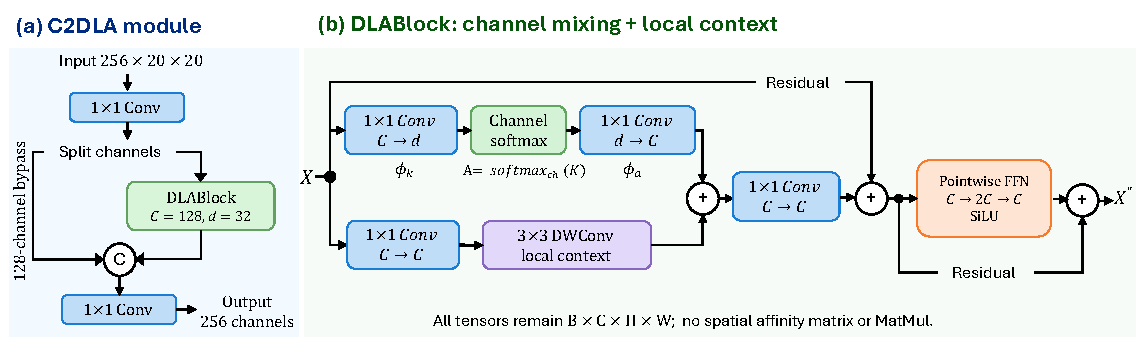
\includegraphics[width=\textwidth]{figures/c2dla_detail.pdf}
\caption{\textbf{C2DLA module and operators.} (a) Nano-model split--process--merge block
 at $20\times20$. (b) Channel softmax and local depthwise convolution replace spatial
 attention, retaining both residual additions and the pointwise FFN.
 C denotes concatenation; $+$ denotes elementwise addition.}
\label{fig:c2dla}
\end{figure*}
\subsection{Design Objective and Verification Criterion}
The workflow treats learned-graph placement as a deployment constraint.
Let $G$ denote the learned graph obtained by adapting the reference YOLO11-n graph.
The objective is to obtain a useful detector whose complete learned computation can run on the tested DLA configuration:
\begin{equation}
 \operatorname{Build}_{\mathrm{DLA}}(G;\theta,\mathrm{fallback}=0)
 = E, \qquad N_{\mathrm{GPU}}(E)=0,
 \label{eq:accept}
\end{equation}
where $\theta$ fixes the target, compiler version, precision, shapes, and
I/O formats, $E$ is the serialized engine, and $N_{\mathrm{GPU}}$ counts
GPU-assigned learned layers after optimization. For this YOLO11 case study, the target is also a single DLA loadable. These are deployment criteria, not training
loss terms. Accuracy and application performance are then evaluated separately.

\subsection{Compatibility Analysis and Adaptation}
Inspection of stock YOLO11-n identifies spatial attention and a flattened, decoded output interface. C2PSA is YOLO11's attention block. It uses a split--process--merge structure in which one branch applies spatial self-attention over the $20\times20$ feature map. This attention requires a query--key MatMul, which strict FP16 compilation rejects. Replacing that learned computation removes the reported blocker. Separately, exporting static raw predictions places the accelerator boundary before decoding and cross-scale output processing. The adaptation therefore uses two substitutions:
\begin{equation}
 \mathrm{C2PSA}\longrightarrow\mathrm{C2DLA},\qquad
 \mathrm{Detect}\longrightarrow\mathrm{DetectDLA}.
 \label{eq:substitutions}
\end{equation}
The surrounding convolutional stem, C3k2 stages, SPPF module, feature-pyramid
connections, detection towers, and ordinary training path are retained
(Fig.~\ref{fig:boundary}). The adapted GPU engine serves as a same-model
placement control. Comparisons with stock YOLO11-n also include architecture,
training, and prediction-interface differences.

\subsection{C2DLA: Replacing Incompatible Spatial Attention}
\label{sec:c2dla}
The replacement must mix information within the processed branch without forming a spatial affinity matrix. C2DLA does this with channel-wise softmax and local depthwise convolution while retaining C2PSA's surrounding split--process--merge structure (Fig.~\ref{fig:c2dla}). An initial $1\times1$
projection produces two channel groups; one bypasses the inner block and the
other is processed before concatenation and a final projection. If $X$ is the
processed group with $C$ channels, define
\begin{align}
 K &= \phi_k(X), \qquad V=\phi_v(X), \label{eq:kv}\\
 A_{bkhw} &= \frac{\exp K_{bkhw}}{\sum_{j=1}^{d}\exp K_{bjhw}},
 \label{eq:chansoftmax}\\
 Z &= \phi_o\bigl(\phi_a(A)+\psi_{3\times3}(V)\bigr),
 \label{eq:mix}\\
 X' &= X+Z, \label{eq:res1}\\
 X'' &= X'+\operatorname{FFN}(X'). \label{eq:res2}
\end{align}
Here $d=\max(\lfloor C/4\rfloor,8)$; $\phi_k:C\to d$,
$\phi_v:C\to C$, $\phi_a:d\to C$, and $\phi_o:C\to C$ are
$1\times1$ projections. The operator $\psi$ is a $3\times3$ depthwise
convolution. The FFN expands channels from $C$ to $2C$, applies SiLU, and
projects back to $C$. Batch normalization accompanies the relevant convolution
modules and is folded into them for inference; $\phi_a$ is a bias-free
convolution without batch normalization.

The nano configuration is shown in Fig.~\ref{fig:c2dla}: one inner block at the
$20\times20$ scale with $C=128$ and $d=32$. No operation introduces matrix
multiplication, head transposes, or normalization over image positions.

The block uses input-dependent channel mixing and local depthwise context.
It does not model long-range spatial affinities. It changes the hypothesis class
and is not algebraically equivalent to C2PSA; greater representational power
is not claimed. Its accuracy is evaluated in Section~\ref{sec:accuracy}.

\subsection{DetectDLA: A Static Prediction Boundary}
\label{sec:boundary}
Stock Detect performs the expectation over the discrete regression distribution used by distribution focal loss (DFL), grid decoding, sigmoid, flattening, and cross-scale concatenation inside the exported graph before producing its fixed decoded output. DetectDLA stops earlier and instead exposes the three raw multi-scale prediction maps, leaving these operations and variable-cardinality filtering and NMS to the host.

For each pyramid level $\ell\in\{3,4,5\}$, the retained regression and
classification towers produce $R_\ell$ and $S_\ell$. DetectDLA exports
\begin{equation}
 P_\ell=\operatorname{Concat}_{C}(R_\ell,S_\ell)
 \in\mathbb{R}^{B\times(4r+n_c)\times H_\ell\times W_\ell},
 \label{eq:packed}
\end{equation}
with $r=16$ regression bins and $n_c=80$ COCO classes. For batch one and
$640\times640$ images, the outputs are $1\times144\times80\times80$,
$1\times144\times40\times40$, and $1\times144\times20\times20$ at strides
8, 16, and 32. They are named \texttt{pred\_p3}, \texttt{pred\_p4}, and
\texttt{pred\_p5}. Classification values are logits; box channels are
unnormalized distributions, not decoded coordinates.

During training and ordinary PyTorch inference, DetectDLA invokes the
inherited Detect path, retaining its losses and assignment behavior. The change
concerns deployment partitioning, not a direct-regression or one-to-one
prediction formulation.

At FP16, the adapted raw output is $1.714\times$ larger than the stock decoded
output, increasing transfer and host-decoding work.

\subsection{Training and Initialization}
The adapted model is initialized from pretrained YOLO11-n weights. Parameters
with matching names and shapes are reused, while unmatched replacement
parameters retain their initialization; all trainable layers are then fine-tuned.
Training uses COCO train2017 for 500 epochs with batch size 32, $640\times640$
inputs, automatic mixed precision (AMP), and standard HSV, geometric,
horizontal-flip, and mosaic augmentation. Stock and adapted models were not
trained with equal budgets, so their comparison evaluates the resulting
deployed detectors rather than an isolated architectural substitution.
